\documentclass{article}
\usepackage{minted}
\usepackage{hyperref}
\usepackage{graphicx}
\usepackage[left=1in, right=1in]{geometry}


\title{Homework 1 Report}
\author{Taylor Berger}

\begin{document}
\maketitle
\section{Synopsis}
\paragraph{} I decided to continue with the work my team did for project 2 and use the AST generator that was already in place. Continuing with the tradition, all work was done in Python 2.7. I implemented a simple lexer using regular expressions to feed into the parser. Most of my time was spent reducing the AST into a concrete syntax tree. The conversion looks incredibly messy and I am not satisfied with the succinctness of the conversion method, but it works and I ran out of time to make it abide any sort of sanity standards.

\section{The AST}
The AST constructor was finished in project 2 with on minor adjustments as I kept coding the homework. The tokens are now suppposed to be pairs of token identifiers and the value of the token. Since variables and numbers don't have a specific value that can be assigned and identified, they token identifiers serve as the additional information that is needed for the parser to identify literals as the same class of tokens. The code is all located in the appendix

\section{Diplaying the AST}
\paragraph{} The AST can be displayed with some utility functions in the file \verb{ast_reductions.py{. After parsing any ll1 grammar into an AST you can do the following to come up with a nice looking AST in a specified png file:

\begin{minted}[linenos=true]{python}
root, _ = parser.ll1_parse(token_stream)
root = reduce_ast(root)
graph = pydot.Dot('Parse Tree', graph_type='digraph')
g, _ = root.pydot_append(graph, 0)
g.write_png(filename)
\end{minted}

Here is an example parse of a small program I used to test 
parsing was happening correctly. This is after the reductions
were done to help improve the quality of the tree.

\begin{figure}
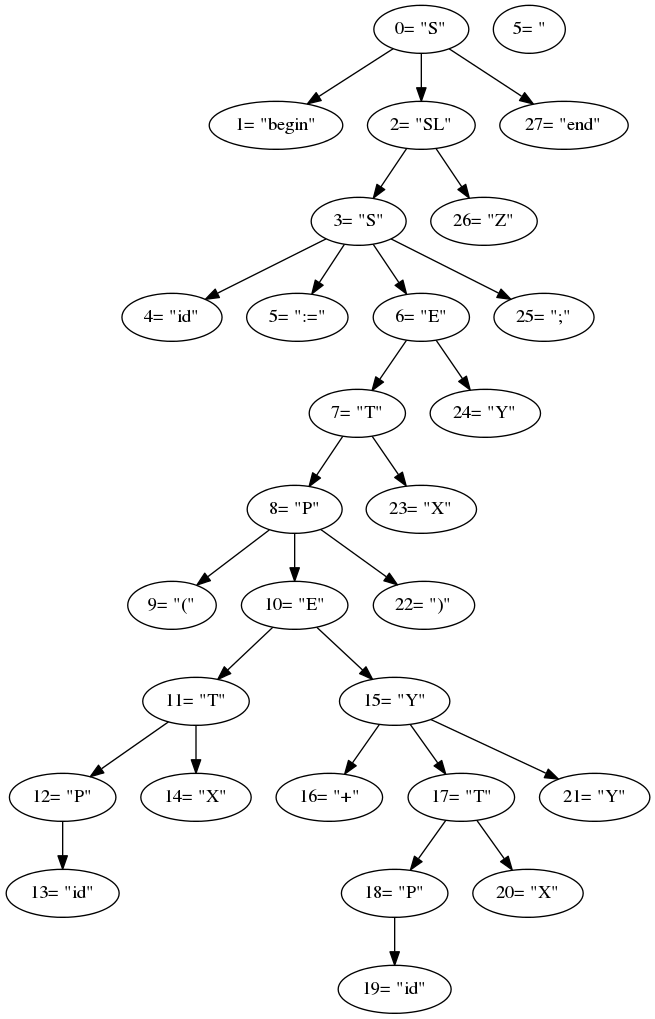
\includegraphics[angle=90,scale=0.2]{../testdata/test.png}
\end{figure}

A better picture can be found \href{https://raw.githubusercontent.com/teberger/cs554-project2/h1_pre_reporty/testdata/test.png}{here}.

\section{Converting to LLVM}
All conversion from a Concrete Syntax tree occurs in the file \verb{ast_to_llvm.py{ and should be viewed in the code appendix immediately following. Once in a Concrete Syntax Tree, the LLVM conversion was very simple -- it follows the CST directly and only two special cases were needed (while and if statements). 

\section{Tieing it All Together}
A testing suite that compiles all pieces together into native code
is provided in \verb{homework1_suite.py{. The file can be run directly on another file that contains the arithmetic language and will output native code. 

\section{Problems and Limitations}
There is a small problem with the Parse Table and grammar representation. For some reason, when constructing the parse table, there are multiple entries in some of the table cells. However using other external tools, the grammar is an LL1 grammar. Upon closer inspection, the parse table tends to have an extra production of the form X -> EPSILON in some of the table's cells. Instead of failing, we try to parse the using the ``left-most'' production (which is the non-epsilon production). Every parsed instance shows that this is perfectly fine and there has been no cases in which the parse fails on a valid grammar when it finds a table's cell with two productions. 
\section*{Code Appendicies}

I'm only including the new code in here that differed from project 2. The other code can be found at my \href{https://github.com/teberger/cs554-project2/tree/h1_pre_reporty}{github}. The minor changes to the other files were excluded since they were minor bug fixes and did not affect the rest of the code.

\subsection{ast\_to\_llvm.py}
\inputminted{python}{../ast_to_llvm.py}
\newpage

\subsection{ast\_reductions.py}
\inputminted{python}{../ast_reductions.py}
\newpage

\subsection{homework1\_suite.py}
\inputminted{python}{../homework1_suite.py}
\newpage

\end{document}
